\chapter{BroodwarBotQ}%: putting it all together}
%%% There's no difference between a pessimist who says, "Oh it's hopeless, so don’t bother doing anything." and an optimist who says, "Don't bother doing anything, it's going to turn out fine anyways. Either way, nothing happens.
%%% --Yvon Chouinard
\label{chapter:bot}


%%% BBQ LOC
%%% cpp:          23234

\begin{quotation}
\textit{Dealing with failure is easy: Work hard to improve. Success is also easy to handled: You've solved the wrong problem. Work hard to improve.}\\
\begin{flushright}Alan J. Perlis (1982)\end{flushright}
\end{quotation}

\lettrine{I}{n} this chapter, we present some of the engineering that went in the robotic player's (bot) implementation. We will also present the different flows of informations and how decisions are made during a game. Finally we will present the results of the full robotic player to various bots competitions.

\ifthenelse{\equal{\myebookformat}{false}}{
\chaptertoc
}{}



\citep{Wolfe11} % BOUNDED INTENTION PLANNING

\section{Code architecture}

\label{sec:codearchitecture}
mapping schéma code <-> schéma info-flow.

\begin{figure}[h]
\begin{center}
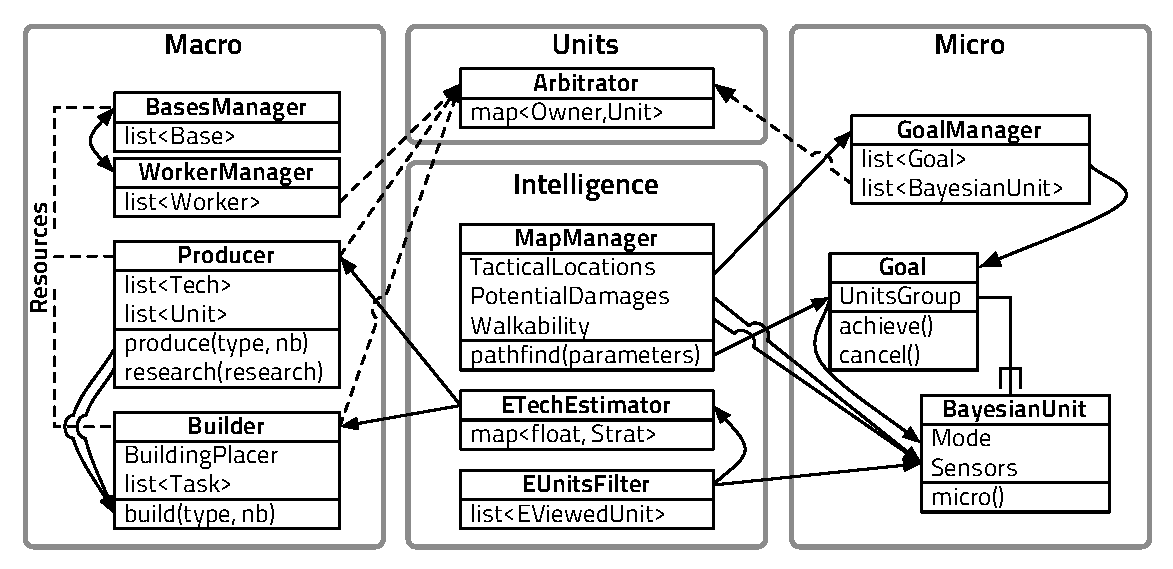
\includegraphics[width=16cm]{images/BBQEarly2012.pdf}
\caption{Simple view of the code architecture of \textsc{BroodwarBotQ}, the most important interactions are shown: every piece which has responsibility for the control of units refer to the \texttt{Arbitrator}, all macro components compete for resources, all other arrows represent orders or important transfers of information.}
\label{fig:codearchitecture}
\end{center}
\end{figure}

\subsection{Tactical goals}
\label{sec:goals}
The decision that we want our AI system to make at this level is \textit{where} and \textit{how} to attack. This is reflected in the StarCraft bot as a \texttt{Goal} creation. \texttt{Goals} are interfacing high level tactical thinking with the steps necessary to their realization. A \texttt{Goal} recruits units and binds them under a \texttt{UnitsGroup} (see section~\ref{sec:unitsgroup}). A \texttt{Goal} is an \glos{FSM} in which two states are simple planners (an FSM with some form of procedural autonomy), it has:
\begin{itemize}
    \item preconditions, for instance a \textit{drop} attack needs to specify at least a transport unit (Shuttle/Dropship/Overlord) and ground attack units.
    \item hard states: \textit{waiting precondition, in progress, in cancel, achieved, canceled}, which corresponds to the \texttt{Goal} advancement..
    \item \textit{and} and/or \textit{or} logic subgoals with:
        \begin{itemize}
            \item a realization test
            \item a proposition of action to try to realize it
            \item an estimation of the ``distance'' to realization
        \end{itemize}
\end{itemize}
In the \textit{in progress} and \textit{in cancel} modes, the ``plan'' is a simple search in the achievable subgoals and their ``distance'' to realization.

The tactical model can specify \textit{where} to attack by setting a localized subgoal (Formation/See/Regroup/KillSubgoal...) to the right place. It can specify \textit{how} by setting the adequate precondition(s).


\section{A game walkthrough}
The tree of decisions.


\section{Results}


BroodwarBotQ took part in the AIIDE 2011 StarCraft AI competition. It got 67 ``crashes'' on 360 games because of a misinterpretation of rules on the first frame\footnote{the additional terrain analysis was not serialized and taking more than one minute on the frame 0, which has no special tolerance as opposed as the year before.}, which is not the real unstability of the bot ($\approx$ 0,75\% as seen in \ref{fig:ladderbots}). The results of AIIDE are in Table~\ref{tab:botsAIIDE}.

\begin{table}[h]
    \begin{center}
    \begin{small}
    \begin{tabular}{|l|l|l|c|l|}
        \hline
        bot & race & refs & win rate & notes \\
        \hline
     Skynet\footnote{\url{http://code.google.com/p/skynetbot/} } & Protoss & & 0.889 & robust openings depending on opponent's race \\
UAlbertaBot & Protoss & \citep{Churchill2011} & 0.794 & always 2-Gates opening \\
       Aiur\footnote{\url{http://code.google.com/p/aiurproject/}} & Protoss & & 0.703 & robust and stochastic strategies \\
ItayUndermind & Zerg & & 0.658 & 6-pooling \\
       EISBot\footnote{\url{http://code.google.com/p/eisbot/}} & Protoss & \citep{WeberCIG10,Weber2010cr} & 0.606 & 2-Gates or Dragoons opening \\
         SPAR\footnote{\url{http://www.planiart.usherbrooke.ca/projects/spar/}} & Protoss & \citep{Kabanza2010} & 0.539 & uses Dark Templars \\
    Undermind & Terran & & 0.517 & Barracks units \\
         Nova\footnote{\url{http://www.planiart.usherbrooke.ca/projects/spar/}} & Terran & \citep{NovaBot2011} &  0.475 & robust play \\
 BroodwarBotQ\footnote{\url{https://github.com/SnippyHolloW/BroodwarBotQ}} & Protoss  & %\citep{SYNNAEVE:OpeningPred} \citep{SYNNAEVE:Micro} 
& 0.328 & adapts to the opening \\
        BTHAI\footnote{\url{http://code.google.com/p/bthai/}} & Zerg & \citep{Hagelback2009} & 0.319 & Lurkers opening  \\
    Cromulent & Terran & & 0.300 & Factory units \\
   bigbrother & Zerg & & 0.278 & Hydralisks and Lurkers \\
       Quorum & Terran & & 0.094 & expands and produce Factory units \\
        \hline
    \end{tabular}
    \end{small}
    \end{center}
    \caption{Result table for the AIIDE 2011 StarCraft AI competition with 360 games played by each bot.}
    \label{tab:botsAIIDE}
\end{table}
%%% AIIDE 2011
%%% Skynet
%%% UAlbertaBot
%%% Aiur
%%% ItayUndermind
%%% EISBot
%%% SPAR
%%% Undermind
%%% Nova
%%% BroodwarBotQ
%%% BTHAI
%%% Cromulent
%%% bigbrother
%%% Quorum

Also in 2011 was the CIG 2011 StarCraft AI competition. It has 10 entries and BroodwarBotQ placed 4th with a little luck of seed (it did not have to play against Aiur). The finals are depicted in Table~\ref{tab:botsCIG}.
\begin{table}[h]
    \begin{center}
    \begin{tabular}{|l|c|c|c|}
        \hline
bot & crashes & games & wins \\ 
Skynet & 0 & 30 & 26 \\ 
UAlbertaBot & 0 & 30 &  22\\
Xelnaga\footnote{A modified version of AIUR doing only Dark Templar rushes.} & 3 & 30 & 11 \\
BroodwarBotQ & 2 & 30 & 1\\
        \hline
    \end{tabular}
    \end{center}
    \caption{Result table of the finals for the CIG 2011 StarCraft AI competition (10 entries)}
    \label{tab:botsCIG}
\end{table}

Finally, there is ladder running in which BroodwarBotQ (last updated January 2012) is ranked between 7 and 9 (without counting duplicates, there are $\approx$ 20 different bots) and is on-par with EISBot \citep{WeberCIG10,Weber2010cr} as can be seen in Figure~\ref{fig:ladderbots} (February 2012 ladder ranking).

